% Chapter 4

\chapter{Topic modeling for sentiment analysis} % Main chapter title

\label{topicmodeledsa} % For referencing the chapter elsewhere, use \ref{Chapter4} 

\lhead{Chapter 4. \emph{Joint Modeling of Sentiment and Topic}} % This is for the header on each page - perhaps a shortened title

%----------------------------------------------------------------------------------------

In this chapter, we will show how topic models are used for \textit{SA}. In the first section, we will show how the basic 
\textit{LDA} model can be used to classify documents based on their polarity.

\section{LDA for sentiment analysis}

Let us first list the basic steps to use any topic model for discovering topics.

\subsection{Using Topic models}

\begin{itemize}
 \itemsep0em
 \item Set number of topics.
 \item Remove stop-words as they do not belong to any topic.
 \item Estimate probabilities using some inference method.
 \item Use the trained model for inference of topics in new documents.
\end{itemize}

\subsection{Using LDA for Sentiment Classification}

To use basic LDA as a sentiment classifier, we add one more step to remove objective words.
Also, usually during Gibbs sampling the first step assigns topics randomly to words. Instead, we
introduce a prior information about the positivity and negativity of words to assign topics to 
words initially. The steps are as follows.

\begin{itemize}
 \itemsep0em
 \item Set number of topics, 2 in this case viz. positive and negative.
 \item Remove stop-words.
 \item Remove objective words as they won't affect sentiment.
 \item Gibbs Sampling with prior using lists of positive and negative words.
 \item Use the trained model to classify a new document as positive or negative.
\end{itemize}

The experimental setup and the results for this approach are discussed in ~\cref{experiments}. The observations made in these
experiments gave way to an approach for resource generation using \textit{LDA}. In the next section, we explain an approach
to do the same.

\section{Resource generation using LDA}

LDA can be used for resource generation of positive and negative words. The steps to do so are explained below.

\begin{itemize}
 \itemsep0em
 \item Set number of topics equal to 3 i.e., positive, negative and objective. We do not remove the objective
 words in this case as we want to find out which of them are positive or negative.
 \item Remove stop-words.
 \item Gibbs Sampling with prior using lists of positive and negative words. In the initial step, words present 
 in the list are assigned that specific topic but the other words as assigned a topic randomly.
 \item Get the top words in the positive and negative topics.
\end{itemize}

The list of positive and negative words we obtained using this approach were used to enhance our systems as show in ~\cref{experiments}.

\section{Joint models of topic and sentiment}

SA has been used in IR to improve the performance. IR was mainly concerned with factual/objective data. So, intuitively we see
that subjectivity classification can aid IR. \citep*{riloff2005exploiting} has work based on it in which they try to exploit
subjectivity analysis to improve performance of information extraction. 

Corpus models are useful in fetching documents specific to a certain topic. Sometimes a user might need to fetch documents which
have a specific sentiment. One such work on sentiment retrieval using generative models is seen in \citep*{eguchi2006sentiment}.
In this work, they have assumed that user inputs both query terms as well as indicates the desired sentiment polarity in some way.
They have combined sentiment and topic relevance models to retrieve documents which are most relevant to such user requests. This
approach is very important for sentiment aware information retrieval.

The expression of sentiment in the text is topic dependent. Negative review for a voting event may be expressed using \textit{flawed}. 
On the other hand negative review of politician may be expressed using \textit{reckless}. Sentiment polarity is topic dependent \citep*{engstrom2004topic}.
The adjective \textit{unpredictable} will have a negative orientation in a car review and it will have a positive orientation in a
movie review. 

\subsection*{Terminology}

The goal of the model is to generate a collection of sentences \(s_1,s_2,\dots,s_n\). Every document is composed of words \(w_1,w_2,\dots,w_n\)
drawn from the vocabulary \(V\). A binary variable \(b_{ij} \in \{S,T\}\) is used to represent whether a word in position \(j\) in 
sentence \(i\) is a topic word or a sentiment word. Let \(x_i\) be the polarity for the sentence \(s_i\). \(x_i\) is a discrete 
random variable with three outcomes \(\{-1,0,+1\}\). A statement \(s_i\) is represented as a set \(\{w_i^s,w_i^t,x_i\}\) where \(w_i^s\) are the
sentiment bearing words, \(w_i^t\) are the topic bearing words and \(x_i\) is the sentence polarity. The user query will be represented
in a similar fashion \(\{q_i^s,q_i^t,q^x\}\). Let \(p\) denote a unigram language model. \(P\) denotes the set of all possible
language models. It is the probability simplex. Similarly, let \(p_x\) denote the distribution over three possible polarity values and
\(P_x\) will be the corresponding ternary probability simplex. The function \(\pi:P \times P \times P_x\to[0,1]\) is a function which 
assigns a probability \(\pi(p_1,p_2,p_x)\) to a pair of language models \(p_1\) and \(p_2\) together with \(p_x\).

\subsection*{Generative model of sentiment}

A sentence \(s_i\) containing words \(w_1,w_2,\dots,w_j,\dots,w_m\) is generated in the following way:

\begin{enumerate}
 \item Draw \textit{p_t, p_s and p_x} from \(\pi (\cdot,\cdot,\cdot)\).
 \item Sample \(x_i\) from a polarity distribution \(p_x(\cdot)\).
 \item For each position \(\textit{j = 1\dots m}\):
  \begin{itemize}
   \item if \(b_{ij}=T\): draw \(w_{j}\) from \(p_t(\cdot)\);
   \item if \(b_{ij}=S\): draw \(w_{j}\) from \(p_s(\cdot)\)
  \end{itemize}
\end{enumerate}

The probability of observing the new statement \(s_i\) containing words \(w_1,w_2,\dots,w_j,\dots,w_m\) is given by:

\begin{equation}
\sum_{p_t,p_s,p_x} \pi(p_t,p_s,p_x)p_x(x_i) \prod_{j=1}^m \left\{ 
  \begin{array}{l l}
    p_t(w_j) & \quad \text{if b_{ij} = T}\\
    p_s(w_j) & \quad \text{otherwise}
  \end{array} \right.
\end{equation}

The probability functions are dirichlet smoothed models and \(\pi(p_1,p_2,p_x)\) is a non-parametric function. 

Each sentence is represented as a bag of words model and the model makes strong independence assumptions. But, due to joint
probability distribution used it is able to model co-occurrence. 

\subsection*{Retrieval using the model}

Suppose we are given a collection of statement \(C\) and a query \(\{q_i^s,q_i^t,q^x\}\) given by the user. The topic relevance model
\(R_t\) and the sentiment relevance model \(R_t\) are estimated. For each word \(w\) in a statement within a collection \(C\), these
models are estimated as follows:


\begin{equation}
R_t(w) = \frac{P(q^s,q^t\circ w,q^x)}{P(q^s,q^t,q^x)} , R_s(w) = \frac{P(q^s \circ w,q^t,q^x)}{P(q^s,q^t,q^x)} 
\end{equation}

\(q \circ w\) means appending \(w\) to the list \(q\). The statements are ranked using a variation of cross-entropy,

\begin{equation}
 \alpha \sum_v R_t(v) \log p_t (v) + (1-\alpha) \sum_v R_s(v) \log p_s(v)
\end{equation}

\par

The experiments using this approach have shown promising results. This shows that sentiment aware IR can benefit from this technique.
As corpus models have been widely used in IR, extending and tuning them for SA aware IR can yield good results. 


\section{Joint Sentiment-Topic modeling (JST)}

\citep*{lin2009joint} discusses a joint model of sentiment and topics. Following figure shows the model.

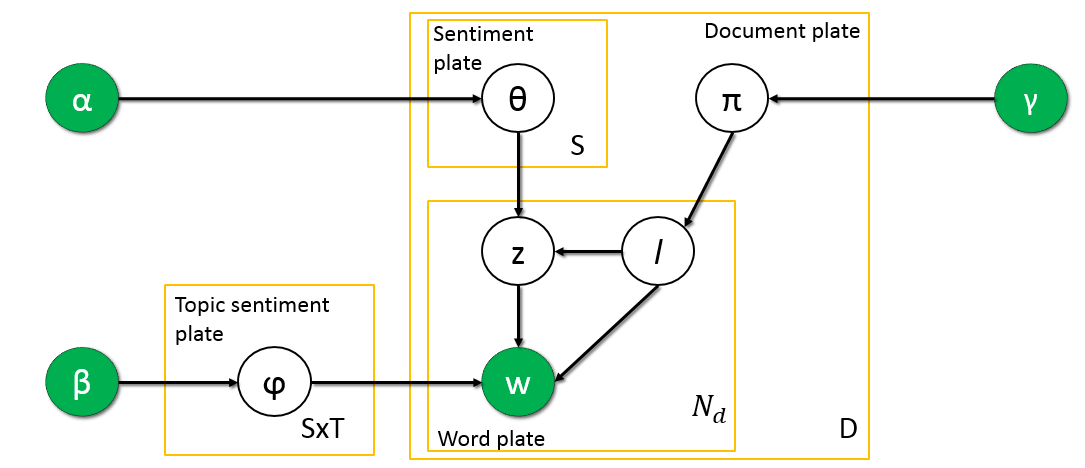
\includegraphics[width=\textwidth]{jst/jst.png} 
\begin{center}
 Figure 4.1 Joint Sentiment Topic Model
\end{center}

Assume that we have a collection of \(D\) documents denoted by \(C = {d_1,d_2,\cdots,d_D} \); each document in the corpus is a sequence
of \(N_d\) words denoted by \(d = (w_1,w_2,\cdots,w_{N_d}) \) and each word in the document is an item from a vocabulary index with V distinct
terms denoted by \({1,2,\cdots,V}\). Let \(S\) and \(T\) be the number of distinct sentiment and topic labels respectively. The procedure of
generating a document is described as follows.

\begin{alltt}
For each document \(d\), choose a distribution \(\pi_d \sim Dir(\gamma)\).
For each sentiment label \(l\) under document \(d\), choose a distribution
\(\theta_{d,k} \sim Dir(\alpha)\).
For each word \(w_i\) in document \(d\)
  - choose a sentiment label \(l_i \sim \pi_d\),
  - choose a topic \(z_i \sim \theta_{d,l_i}\),
  - choose a word \(w_i\) from the distribution over words defined by the 
    topic \(z_i\) and sentiment label \(l_i\), \(\psi_{z_i}^{l_i}\)
\end{alltt}

The hyper-parameter \(\alpha\) in \textit{JST} is the prior observation count for the number of times topic \(j\) is associated with 
sentiment label \(l\) sampled from a document. 

The hyper-parameter \(\beta\) is the prior observation count for the number of times words sampled from topic \(j\)
are associated with sentiment label \(l\).

Similarly, the hyper-parameter \(\gamma\) is the prior observation count for the number of times sentiment label \(l\) is associated
with a document.

The latent variables of interest in \textit{JST} are
\begin{enumerate}
 \item The joint sentiment/topic-document distribution, \(\theta\)
 \item The joint sentiment/topic-word distribution, \(\phi\)
 \item The joint sentiment-document distribution, \(\pi\)
\end{enumerate}

To obtain the distributions for \(\theta\), \(\phi\), and \(\pi\), we firstly estimate the posterior distribution over \(z\) i.e, the assignment
of word tokens to topics and sentiment labels.

We need to estimate the distribution, \(P(z_t=j,l_t=k|w,z_{\neg t},l_{\neg t},\alpha,\beta,\gamma)\) where \(z_{\neg t}\) and \(l_{\neg t}\)
are vector of assignments of topics and labels for all words in the collection except for the word position \(t\) in document \(d\). 

The joint distribution can be given as follows,
\begin{equation}
P(w,z,l) = P(w|z,l)P(z|l) = P(w|z,l)P(z|l,d)P(l|d)
\end{equation}

After calculations similar to \textit{LDA}, we get the following full conditional,

\begin{equation}
P(z_t=j,l_t=k|w,z_{\neg t},l_{\neg t},\alpha,\beta,\gamma) = 
\frac{\{N_{i,j,k}\}_{\neg t} + \beta}{\{N_{j,k}\}_{\neg t}+V\beta}.
\frac{\{N_{j,k,d}\}_{\neg t} + \alpha}{\{N_{k,d}\}_{\neg t}+T\alpha}.
\frac{\{N_{k,d}\}_{\neg t} + \gamma}{\{N_{d}\}_{\neg t}+S\gamma}
\end{equation}

where,

\(V\) is the size of the vocabulary \\
\(T\) is the number of topics \\
\(S\) is the total number of sentiment labels \\
\(D\) is the number of documents in the collection \\
\(N_{i,j,k}\) is the number of times word \(i\) appeared in topic \(j\) and with sentiment label \(k\) \\
\(N_{j,k}\) is the number of times words are assigned to topic \(j\) and sentiment label \(k\) \\
\(N_{j,k,d}\) is the number of times a word from document \(d\) has been associated with topic \(j\) and sentiment label \(k\) \\
\(N_{k,d}\) is the number of times sentiment label \(k\) has been assigned to some word tokens in document \(d\) \\
\(N_{d}\) is the total number of words in the collection \\

\par

\(\theta\), \(\phi\), and \(\pi\) can be estimated as follows

\begin{equation}
\phi_{i,j,k} = \frac{N_{i,j,k}+\beta}{N_{j,k}+V\beta}
\end{equation}

\begin{equation}
\theta_{j,k,d} = \frac{N_{j,k,d}+\alpha}{N_{k,d}+T\alpha}
\end{equation}

\begin{equation}
\pi_{k,d} = \frac{N_{k,d}+\gamma}{N_{d}+S\gamma}
\end{equation}

The Gibbs sampling procedure in this case is similar to that of \textit{LDA}. 

\par
\textit{JST} can be used for document level sentiment classification and topic detection simultaneously. \textit{Joint sentiment topic modeling}
is completely unsupervised as compared to existing approaches for sentiment classification. The performance of \textit{JST} on movie review
classification is competitive compared to other supervised approaches. \textit{JST} has been used in our experiments to compare it against our
approaches for sentiment analysis as explained in \cref{experiments}.

\section*{Summary}
In this chapter we explained how basic LDA can be used to perform the sentiment classification task. We also studied two models which combine sentiment
and topics. Both the systems have shown high competence in classification tasks. In the next chapter, we discuss the the topical n-gram model in detail.
We also explain how it can be used for sentiment classification.

\clearpage